\documentclass[tikz, border=5mm]{standalone}
\usepackage{amsmath, amssymb}
\usetikzlibrary{arrows.meta, decorations.markings, calc, patterns}

% Define styles for consistency
\tikzset{
	boundary style/.style={
		line width=2pt,
		blue!70!black,
		postaction={decorate},
		decoration={
			markings,
			mark=between positions 0.1 and 1 step 0.2 with {\arrow[scale=1.5]{>}}
		}
	},
	interior curl style/.style={
		orange!80!red,
		thin,
		{<[scale=0.8]}-{>[scale=0.8]}
	},
	vector field style/.style={
		gray!30,
		dashed,
		->,
		shorten >=2pt,
		shorten <=2pt
	}
}

\begin{document}
	
	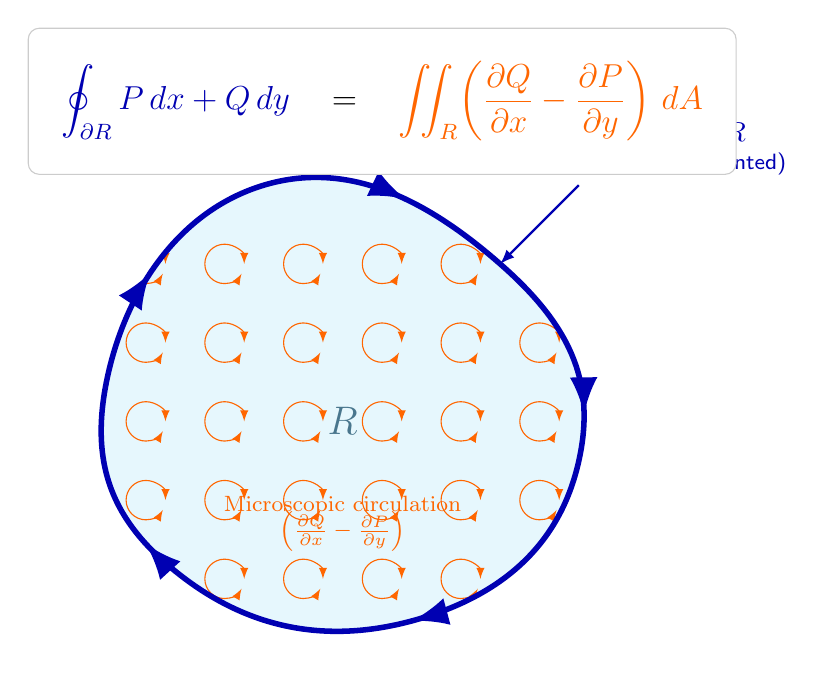
\begin{tikzpicture}[>=latex, font=\sffamily]
		
		% --- 1. Define the Region Path ---
		% A smooth, arbitrary closed shape
		\def\regionpath{
			plot [smooth cycle, tension=0.8] coordinates {
				(0, 1) (2, 3.5) (5, 2.5) (6, 0) (4, -2) (1, -1.5)
			}
		}
		
		% --- 2. Draw Faint Vector Field Background (Optional Context) ---
		% Suggests the field F = <P,Q> exists everywhere
		\begin{scope}
			\clip \regionpath; % Clip field to inside the region for cleaner look
			\foreach \x in {0, 0.8, ..., 6} {
				\foreach \y in {-2, -1.2, ..., 3.5} {
					% Simple arbitrary field for visualization: (y, -x/2) roughly
					\draw[vector field style] (\x,\y) -- ++({\y/4}, {-\x/8});
				}
			}
		\end{scope}
		
		
		% --- 3. Fill the Region R ---
		\fill[cyan!10] \regionpath;
		
		
		% --- 4. Visualize the RHS: Interior Micro-Curls ---
		% Draw a grid of small counter-clockwise arrows representing the curl
		\begin{scope}
			\clip \regionpath; % Ensure small arrows stay inside
			\foreach \x in {0.5, 1.5, ..., 5.5} {
				\foreach \y in {-1.5, -0.5, ..., 3} {
					\begin{scope}[shift={(\x,\y)}]
						% Draw a small incomplete circle with arrows
						% to represent local rotation density (curl)
						\draw[interior curl style] (0.25, 0) arc (0:330:0.25);
					\end{scope}
				}
			}
		\end{scope}
		
		
		% --- 5. Visualize the LHS: The Boundary Line Integral ---
		\draw[boundary style] \regionpath;
		
		
		% --- 6. Labels ---
		% Label the region R
		\node[font=\Large, cyan!50!black] at (3, 0.5) {$R$};
		
		% Label the boundary dR using a pin line for clarity
		\coordinate (BoundaryPoint) at (5, 2.5);
		\draw[<-, blue!70!black, thick] (BoundaryPoint) -- ++(1, 1) 
		node[above right, align=left] {Boundary $\partial R$\\[-0.2em]\footnotesize (Positively oriented)};
		
		% Label the interior curl concept
		\node[orange!80!red, align=center, font=\footnotesize] at (3, -0.8) {
			Microscopic circulation\\[-0.3em] $\left(\frac{\partial Q}{\partial x}-\frac{\partial P}{\partial y}\right)$
		};
		
		
		% --- 7. The Theorem Equation Box ---
		\node[
		anchor=north west, 
		fill=white, 
		draw=gray!40, 
		rounded corners, 
%		drop shadow, 
		inner sep=12pt,
		font=\large
		] at (-1, 5.5) {
			% Color-coding the equation to match the diagram
			$\displaystyle 
			\color{blue!70!black}
			\oint_{\partial R} P\,dx+Q\,dy
			\color{black}
			\quad = \quad
			\color{orange!80!red}
			\iint_R\!\left(\frac{\partial Q}{\partial x}-\frac{\partial P}{\partial y}\right)\,dA$
		};
		
	\end{tikzpicture}
	
\end{document}